\chapter{L3:  Abstract Syntax Trees and Natural Deduction Proof Outlines}

\begin{quote}
	\begin{center}
	Standard L3
	\end{center}
	\medskip 
	
	I can make the Abstract Syntax Tree (AST) for a statement.  I can use the AST to generate a natural deduction proof outline.  I can complete these proof outlines to give proofs of more complicated theorems about equalities, inequalities, parity, and divisibility.  
	\end{quote}
\section{Syntax Trees}

We have already proven some fairly complex logical statements.  You may have found that it is sometimes difficult to determine which \textbf{order} to apply the introduction and elimination rules in.  In this chapter we learn about an organizational tool called an \index{abstract syntax tree}\textbf{abstract syntax tree} (AST for short) which helps us understand how to order our structured proof outlines. 

In  chapter 2  we analyzed the following two propositions:

\begin{enumerate}
	\item $\exists x \in \mathbb{R}: [(2x+1 = 5) \wedge (3x+3 = 5)]$
	
	\item $[\exists x \in \mathbb{R}: (2x+1 = 5)] \wedge [\exists x: (3x+3 = 5)]$
\end{enumerate}

Understanding the difference between these two statements may have been difficult for you.  The AST  might be a little easier to understand (once you get the hang of it).

Statement (1) is existentially quantifying the predicate $[(2x+1 = 5) \wedge (3x+3 = 5)]$ in the variable $x$.  I will record this by having the \textbf{root node} of the syntax tree be $\exists x \in \mathbb{R}$, drawing a single vertical \textbf{branch} down from that node and then putting the syntax tree for the predicate $[(2x+1 = 5) \wedge (3x+3 = 5)]$ below it:

\begin{center}
	\begin{forest}
		[\(\exists x \in \mathbb{R}\)[Tree for ``\({(2x+1 = 5) \wedge (3x+3 = 5)}\)'']]
	\end{forest}
\end{center}

Since the predicate $[(2x+1 = 5) \wedge (3x+3 = 5)]$ is a conjunction of the two predicates $2x+1 = 5$ and $3x+3 = 5$, the tree for this predicate will have a root of $\wedge$, two branches, with $2x+1 = 5$ on the left and $3x+3 = 5$ on the right:

\begin{center}
	\begin{forest}
		[\(\exists x \in \mathbb{R}\)[\(\wedge\)[\({2x+1 = 5}\)][\({3x+3 = 5}\)]]]
	\end{forest}
\end{center}

The  final \textbf{leaves} at the bottom of this tree do not contain any logical connectives or quantifiers.  Each variable appearing in the leaves can be traced back to a single quantifier which introduces the variable.

However, the syntax tree for (2) would look like:

\begin{center}
	\begin{forest}
		[\(\wedge\)[\(\exists x \in \mathbb{R}\)[\( {2x+1 = 5}\)]][\(\exists x \in \mathbb{R}\)[\( {3x+3 = 5}\)]]]
	\end{forest}
\end{center}

Note that the ``tree'' analogy is a bit strange since it is upside down!  The root is at the top, and the leaves are at the bottom!  The reason for this strange convention is that we usually like to work from top to bottom when writing on a page in English.

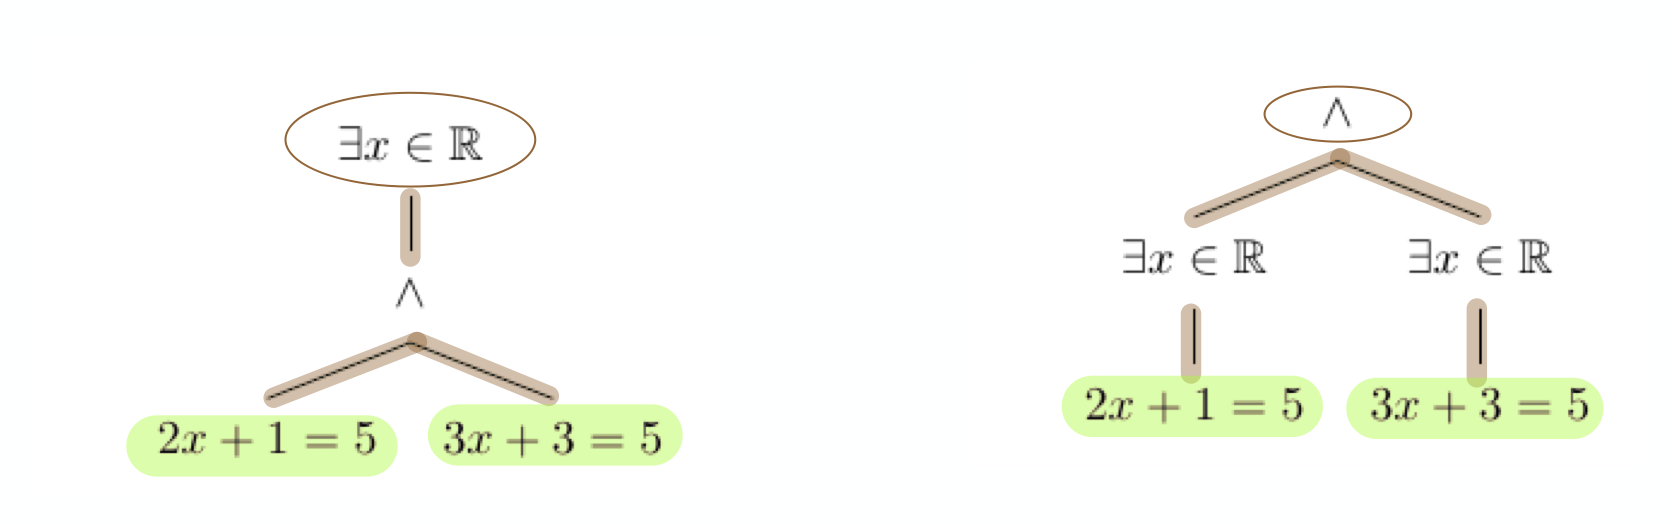
\includegraphics[scale = 0.4]{trees}

Here the root is circled, the branches are colored brown, and the leaves are colored green.

Comparing these two we see that in (1) the existential quantification of $x$ applies to both statements $2x+1 = 5$ and $3x+3  = 5$.  We would say that both instances of $x$ are within the \index{scope}\textbf{scope} of this existential quantifier.  However, in (2) the scope of the exitential quantifier on the left branch only includes the $x$ in $2x+1  = 5$, while the scope of the existential quantifier on the right branch only includes the $x$ in $3x+3 = 5$.

\begin{example}
	Assume that $p$ is a proposition while $A$, $B$, and $C$ are predicates. The syntax tree for 
	
	\[
	\exists x :[( P \wedge A(x)) \wedge ( \forall y( B(x) \wedge C(x,y) ))]
	\]
	
	is
	
	\begin{center}
		\begin{forest}
			[\(\exists x\)[\(\wedge\)[\(\wedge\)[\(P\)][\(A(x)\)]][\(\forall y \)[\(\wedge\)[\(B(x)\)][\({C(x,y)}\)]]]]]
		\end{forest}
	\end{center}
	
	The two dimensional layout of the tree makes some features of the expression easier to parse than when we leave it as a one dimensional written expression.
\end{example}

\begin{xca}
	Build a syntax tree for each of the following statements.  Assume that $p$, $q$, and $r$ are propositions and $A$, $B$, and $C$ are predicates.  Matching parenthesis can be a struggle:  this is part of the reason why trees can be a useful way of writing these expressions.  Then categorize the sentence according to its root node.
	
	\begin{enumerate}
		\item $\forall x:  p \wedge \exists y :(A(x,y) \wedge B(x)))$
		\item $p \wedge (q \wedge \exists t: (B(t,t)) )$
		\item $\forall x: ( \exists y (A(x,y)) \wedge \forall y: (C(x,y)))$
	\end{enumerate}
\end{xca}


\begin{solutions}
	\begin{enumerate}
		\item $\forall x:  (p \wedge \exists y: (A(x,y) \wedge B(x)))$
		
		\begin{center}
			\begin{forest}
				[\(\forall x\)[\(\wedge\)[\(p\)][\(\exists y\)[\(\wedge\)[\({A(x,y)}\)][\(B(x)\)]]]]]
			\end{forest}
		\end{center}
	

	
		\item $p \wedge (q \wedge \exists t: (B(t,t)) )$
		
		\begin{center}
			\begin{forest}
				[\(\wedge\)[\(p\)][\(\wedge\)[\(q\)][\(\exists t\)[\({B(t,t)}\)]]]]
			\end{forest}
		
		\end{center}
		\item $\forall x: ( \exists y (A(x,y)) \wedge \forall y (C(x,y)))$
		
		\begin{center}
			\begin{forest}
				[\(\forall x\)[\(\wedge\)[\(\exists y\)[\({A(x,y)}\)]][\(\forall y\)[\({C(x,y)}\)]]]]
			\end{forest}
	
		\end{center}
		
	\end{enumerate}
\end{solutions}

\begin{xca}
	Consider the syntax tree
	
	\begin{center}
		\begin{forest}
			[$\forall x$[$\wedge$[$\exists y$[${A(x,y)}$]][$\forall y$[$\wedge$[$p$][${B(x,y)}$]]]]]
		\end{forest}
	\end{center}
	
	Indicate all variables which are in the scope of $\forall y$.  Then convert this syntax tree to a linear string with appropriate parentheses. 
	
\end{xca}

\begin{solutions}
	The only variable within the scope of $\forall y$ is the $y$ in $B(x,y)$.
	
	We can write this proposition on one line as
	
	\[
	\forall x: (  (\exists y: ( A(x,y)))  \wedge (\forall y: ( p \wedge  B(x,y)))  )
	\]
	
\end{solutions}

\section{Natural Deduction Proof Outlines}

We have seen that we can make the logical structure of mathematical statements clearer by translating them into symbolic form.  That is to say, if we declare the meaning of sentences like $p$, $q$, $r$,  and predicates like $A(x)$,  $B(x)$,  $C(x,y)$, then we can use the logical connectives $\wedge$, $\implies$, $\bi$, $\neg$, $\vee$ and the quantifiers $\forall$ and $\exists$ to translate mathematical statements in English into more formal and precise statements using these symbols.

For example, if we let $E(x)$ be the predicate ``$x$ is even'', then we can translate the English mathematical sentence 

{ \begin{center}
		``The product of any two even numbers is even.''
		\end{center}
}

into a symbolic form where its logical structure is more apparent:

$$
\forall x \in \Z \, \forall y \in \Z \left( E(x) \wedge E(y) \implies E(x+y) \right)
$$

or as a syntax tree:

\begin{center}
\begin{forest}
	[$\forall x \in \Z$[$\forall y \in \Z$[$\implies$[$\wedge$[$E(x)$][$E(y)$]][$E(x+y)$]]]
]
\end{forest}
\end{center}

We will see how to use this logical structure to make a ``Natural Deduction Proof Outline''  for the theorem.  We will generate this outline recursively, moving down the tree.  Proving theorems in mathematics requires considerable creativity, but that creativity often lives in the ``blank spaces'' of this outline, not in the structure of the outline itself.  For each of the five connectives, and two quantifiers, we will use our elimination and introduction rules to guide us in crafting the outline.

Now lets see how to make a proof outline for 

$$
\forall x \in \Z \, \forall y \in \Z \left( E(x) \wedge E(y) \implies E(x+y) \right)
$$

\begin{center}
	\begin{forest}
		[$\forall x \in \Z$[$\forall y \in \Z$[$\implies$[$\wedge$[$E(x)$][$E(y)$]][$E(x+y)$]]]
		]
	\end{forest}
\end{center}

The root of the tree is $\forall x \in \Z$, so (looking at the introduction rule for universal quantifiers) our argument should look like this:

\begin{fitch}
		\textrm{Let $x_1 \in \Z$ be arbitrary} & start $\forall$-intro\\
		\textrm{Prove $\forall y \in \Z \left( E(x_1) \wedge E(y) \implies E(x_1+y) \right)$}\\
	\end{fitch}

How do we prove $\forall y \in \Z \left( E(x_1) \wedge E(y) \implies E(x_1+y) \right)$?  We make a syntax tree and follow the table!

\begin{center}
	\begin{forest}
		[$\forall y \in \Z$[$\implies$[$\wedge$[$E(x_1)$][$E(y)$]][$E(x_1+y)$]]]
	\end{forest}
\end{center}

The root of this tree is also a universal quantifier.  So our argument now looks like this:

\begin{fitch}
	\textrm{Let $x_1 \in \Z$ be arbitrary} & start $\forall$-intro\\
	\textrm{Let $y_1 \in \Z$ be arbitrary}& start $\forall$-intro\\ 
	\textrm{Prove $\left( E(x_1) \wedge E(y_1) \implies E(x_1+y_1) \right)$}\\
\end{fitch}

Now $\left( E(x_1) \wedge E(y_1) \implies E(x_1+y_1) \right)$ has tree

\begin{center}
	\begin{forest}
	[$\implies$[$\wedge$[$E(x_1)$][$E(y)$]][$E(x_1+y)$]]
	\end{forest}
\end{center}

whose root node is implication.  Following the introduction rule for implication, we have

\begin{fitch}
	\textrm{Let $x_1 \in \Z$ be arbitrary}& start $\forall$-intro\\
	\textrm{Let $y_1 \in \Z$ be arbitrary}& start $\forall$-intro\\ 
	\textrm{Assume $E(x_1) \wedge E(y_1)$} & start $\implies$-intro\\
	\fa \textrm{ Prove  $E(x_1+y_1)$}\\
\end{fitch}

Let's use the conjunction elimination rule to spell out exactly what we are allowed to use in our argument:

\begin{fitch}
	\textrm{Let $x_1 \in \Z$ be arbitrary}& start $\forall$-intro\\
	\textrm{Let $y_1 \in \Z$ be arbitrary}& start $\forall$-intro\\ 
	\textrm{Assume $E(x_1) \wedge E(y_1)$}& start $\implies$-intro\\
	\fa E(x_1) & $\wedge$-elim (left)\\
	\fa E(y_1) & $\wedge$-elim (right)\\
	\fa \textrm{Prove  $E(x_1+y_1)$}\\
\end{fitch}

This is a natural deduction outline for the theorem!

Let's do a few more examples which are entirely abstract.

\begin{example}
		We will make a natural deduction outline for a theorem of the form
		
		\[
		\forall t: \exists s: [ A(t,s) \bi (P(t) \vee Q(s))]
		\]
		
		First we make the syntax tree:
		
		\begin{center}
				\begin{forest}
						[$\forall t$ [ $\exists s$ [$\bi$ [${A(s,t)}$][$\vee$[$P(t)$][$Q(s)$]]] ]]
					\end{forest}
			\end{center}


We build the proof outline in stages.  The current root is universal quantification.

\begin{fitch*}
		\textrm{Let $t_1$ be arbitrary.} & start $\forall$-intro\\
		\textrm{Prove $\exists s [ A(t_1,s) \bi (P(t_1) \vee Q(s))]$}
	\end{fitch*}

The root of what we are trying to prove is now existential quantification.

\begin{fitch*}
	\textrm{Let $t_1$ be arbitrary.}& start $\forall$-intro\\
	\textrm{Construct a candidate $s_1$ (which might depend on the choice of $t_1$).} & start $\exists$-intro\\
	\textrm{Prove $A(t_1,s_1) \bi (P(t_1) \vee Q(s_1))$}\\
\end{fitch*}

The root of what we are trying to prove is now a biconditional.

\begin{fitch}
	\textrm{Let $t_1$ be arbitrary.}& start $\forall$-intro\\
\textrm{Construct a candidate $s_1$ (which might depend on the choice of $t_1$).} & start $\exists$-intro\\
	\textrm{Assume $A(t_1,s_1)$} & forward $\implies$-intro\\
	\fa \textrm{Prove $P(t_1) \vee Q(s_1)$}\\
	\textrm{Assume $P(t_1) \vee Q(s_1)$} & backwards $\implies$-intro\\
	\fa \textrm{Prove $A(t_1,s_1)$}
\end{fitch}

\medskip

We have work to do in line $4$.  The objective in line $4$ is a disjunction, so we need to either prove one or the other.  Since we have no idea what these propositions actually are, we cannot decide which one to prove in this case.  So we will just choose one for illustrative purposes.

We can also spell out how we will use the disjunction in line $5$.  This becomes a case analysis, where we need to prove $A(t_1,s_1)$ in both cases.  

\begin{fitch}
	\textrm{Let $t_1$ be arbitrary.}& start $\forall$-intro\\
\textrm{Construct a candidate $s_1$ ( might depend on $t_1$).} & start $\exists$-intro\\
\textrm{Assume $A(t_1,s_1)$} & forward $\bi$-intro\\
	\fa \textrm{Prove $P(t_1)$}\\
	\fa P(t_1) \vee Q(s_1) & $\vee$-intro (left)\\
	\textrm{Assume $P(t_1) \vee Q(s_1)$} & backwards $\bi$-intro\\
	\fa \textrm{Case 1:  Assume $P(t_1)$} & $\vee$-elim case 1\\
	\fa \fa \textrm{Prove $A(t_1,s_1)$}\\
	\fa \textrm{Case 2:  Assume $Q(s_1)$}& $\vee$-elim case 2\\
    \fa \fa \textrm{Prove $A(t_1,s_1)$}\\
    \fa A(t_1,s_1) & $\vee$-elim, 7, 9\\
    A(t_1,s_1) \bi (P(t_1) \vee Q(s_1)) & finish $\bi$-intro 3, 6\\
    \exists s: A(t_1,s) \bi (P(t_1) \vee Q(s)) & finish $\exists$-intro with $s=s_1$, 2\\
	\forall t: \exists s: [ A(t,s) \bi (P(t) \vee Q(s))] & finish $\forall$-intro, 1
\end{fitch}

\textbf{Note}:  line $4$ could have instead said ``Prove $Q(s_1)$'' if that was more appropriate in proving the particular statement of this form we were grappling with.

This proof outline is now complete!

	\end{example}

Lets do another example.  This time we will be less methodical:  you should practice translating from the sentence, to the tree, to the proof outline without using the table.  These elimination and introduction strategies should become fully integrated into your understanding of what the connectives and quantifiers mean.

\begin{example}
		\[
		\forall x:  [ P(x) \implies (\exists y: \neg Q(x,y))]
		\]
	\end{example}

\begin{center}
		\begin{forest}
				[$\forall x$ [$\implies$ [$P(x)$][$\exists y$ [$\neg$ [${Q(x,y)}$]]]]]
			\end{forest}
	\end{center}

\begin{fitch}
		\textrm{Let $x_1$ be arbitrary.} & start $\forall$-intro\\
		\textrm{Assume $P(x_1)$.} & start $\implies$-intro\\
		\fa \textrm{Construct a candidate $y_1$ ( might depend on $x_1$)} & start $\exists$-intro\\
		\fa \textrm{Assume $Q(x_1,y_1)$} & start $\neg$ intro\\
		\fa \fa \textrm{Derive an absurdity (Prove $\bot$).}\\
		\fa \neg Q(x_1,y_1) & finish $\neg$ intro, 4\\
		\fa \exists y : Q(x_1,y) & finish $\exists$ -intro with $y = y_1$, 3\\
		P(x_1) \implies \exists y : Q(x_1,y) & finish $\implies$-intro, 2\\
			\forall x:  [ P(x) \implies (\exists y: \neg Q(x,y))] & finish $\forall$-intro, 1
	\end{fitch}


\begin{example}
		\[
		(\neg \forall x: P(x)) \wedge (\exists x: Q(x))
		\]


\begin{center}
		\begin{forest}
				[$\wedge$[$\neg$[$\forall x$[$P(x)$]]][$\exists x$[$Q(x)$]]]
			\end{forest}
	\end{center}

\begin{fitch}
		\textrm{Assume $\forall x: P(x)$} & start $\neg$ intro\\
		\fa \textrm{Can use that $P(x_1)$ is true for any $x_1$ we choose.} & $\forall$-elim\\
		\fa \textrm{Derive an absurdity.}\\
		\neg  \forall x: P(x) & finish $\neg$ intro, 1\\
		\textrm{Construct a candidate $x_2$.} & start $\exists$-intro\\
		\textrm{Prove $Q(x_2)$.} & finish $\exists$-intro, 5\\
				(\neg \forall x: P(x)) \wedge (\exists x: Q(x)) & $\wedge$-intro, 4, 6
	\end{fitch}
	\end{example}

\section{Proving some more complicated theorems}

We can now construct proof outlines for arbitrary sentences!  For the rest of this course we will be focused on proving theorems about mathematical objects of interest.  Here is a sample of the kinds of theorems we will prove:

\begin{enumerate}
		\item If $x$ is a real number then $x^2 = 1$ if and only if $x=1$ or $x=-1$.
		\item If $a$ is odd, and $b$ is odd, then $a+b$ is even.
		\item For every positive real number $x$, there is a real number $y$ so that if $t$ is a real number with $0<t<y$ then $0<t^2<x$.
\end{enumerate}

We did already prove theorems which were this complicated in Chapter 2.  The tools of this chapter (abstract syntax trees and natural deduction proof outlines) only exist to make it a more systematic process.  It takes any guesswork out of knowing exactly how to structure your argument.

Let's create proof outlines for each of these. 
\medskip

\begin{theorem}
		If $x$ is a real number then $x^2 = 1$ if and only if $x=1$ or $x=-1$.
	\end{theorem}
	
	You probably learned this theorem in high school algebra.  It is the real reason you put $\pm$ signs when you take square roots.  Even though you know this theorem is true, and use it frequently, you have probably never seen a proof.  
	
	Let's prove it!

We can translate this statement into symbolic logic as follows:

\[
\forall x \in \mathbb{R} : [ ({x^2 = 1}) \iff [({x=1}) \vee ({x=-1})] ]
\]

The syntax tree is

\begin{center}
		\begin{forest}
				[\(\forall x \in \mathbb{R}\)[\(\iff\)[\({x^2 = 1}\)][\(\vee\)[\({x=1}\)][\({x=-1}\)]]]]
			\end{forest}
	\end{center}


To construct the proof outline, we move recursively down the tree.  I will do this in \textbf{excruciating} detail.  You want to get to the point where you can easily write down the proof outline without working methodically like this.

The root node is a universal quantifier, so we start with that proof outline.

\begin{fitch}
	\textrm{Let $a \in \mathbb{R}$ be arbitrary.} & start $\forall$-intro\\
	\textrm{Prove $({a^2 = 1}) \iff [({a=1}) \vee ({a=-1})]$ is true. }
	\end{fitch}

The statement in line 2 is a biconditional, so to prove it we need to argue the forwards and backwards implications:

\begin{fitch}
	\textrm{Let $a \in \mathbb{R}$ be arbitrary.}& start $\forall$-intro\\
	\textrm{Assume $a^2 = 1$ is true.} & forwards $\bi$-intro\\
	\fa \textrm{Prove $(a=1) \vee (a=-1)$ is true.}\\
	\textrm{Assume $(a=1) \vee (a=-1)$ is true.} & backwards $\bi$-intro\\
	\fa \textrm{Prove $a^2 = 1$ is true.}
\end{fitch}

In the forwards part since we know that every real number is either positive, negative, or $0$, we can initiate a case analysis depending on the status of $a$.   

In the backwards part we use a case analysis as well.

\begin{fitch}
	\textrm{Let $a \in \mathbb{R}$ be arbitrary.}& start $\forall$-intro\\
	\textrm{Assume $a^2 = 1$ is true.} & forwards $\bi$-intro\\
		\fa \textrm{Case 1: Assume $a > 0$} & $\vee$-elim\\
			\fa \fa \textrm{Argue that $(a=1) \vee (a=-1)$}\\
		\fa \textrm{Case 2: Assume $a < 0$} & $\vee$-elim\\
			\fa \fa \textrm{Argue that $(a=1) \vee (a=-1)$}\\
		\fa \textrm{Case 3: Assume $a = 0$}& $\vee$-elim\\
			\fa \fa \textrm{Argue that $(a=1) \vee (a=-1)$}\\
	\textrm{Assume $(a=1) \vee (a=-1)$ is true.}& backwards $\bi$-intro\\
		\fa  \textrm{Case 1: Assume $a=1$} & $\vee$-elim case 1\\
		\fa \fa \textrm{Argue $a^2 = 1$ is true.}\\
		\fa  \textrm{Case 2: Assume $a=-1$} & $\vee$-elim case 2\\
		\fa \fa \textrm{Argue $a^2 = 1$ is true.}
\end{fitch}

To argue the disjunctions on lines 4, 6, and 8, we will need to prove either the left or right disjunct.  Looking at what case I am in, I have made a judicious choice.  To argue that $a^2=1$ in line 10, we will need to \textbf{use} the disjunction we assumed in line 9.  This is another case analysis:

\begin{fitch}
	\textrm{Let $a \in \mathbb{R}$ be arbitrary.}& start $\forall$-intro\\
	\textrm{Assume $a^2 = 1$ is true.} & forwards $\bi$-intro\\
	\fa \textrm{Case 1: Assume $a > 0$} & $\vee$-elim\\
	\fa \fa  \textrm{Argue that $a=1$}\\
	\fa \fa \textrm{Conclude that $(a=1) \vee (a=-1)$} &$\vee$-intro left\\
	\fa \textrm{Case 2: Assume $a < 0$} &$\vee$-elim\\
	\fa \fa  \textrm{Argue that $a=-1$}\\
	\fa \fa \textrm{Conclude that $(a=1) \vee (a=-1)$} &$\vee$-intro right\\
	\fa \textrm{Case 3: Assume $a = 0$} &$\vee$-elim\\
	\fa \fa  \textrm{Argue that $a=1$}\\
	\fa \fa \textrm{Conclude that $(a=1)  \vee (a=-1)$} & $\vee$-intro left\\
	\textrm{Assume $(a=1) \vee (a=-1)$ is true.}& backwards $\bi$-intro\\
\fa  \textrm{Case 1: Assume $a=1$} & $\vee$-elim case 1\\
\fa \fa \textrm{Argue $a^2 = 1$ is true.}\\
\fa  \textrm{Case 2: Assume $a=-1$} & $\vee$-elim case 2\\
\fa \fa \textrm{Argue $a^2 = 1$ is true.}
\end{fitch}


This is the complete proof outline!

We can now fill in the remaining arguments to have a proof of the theorem:

\begin{fitch}
	\textrm{Let $a \in \mathbb{R}$ be arbitrary.}& start $\forall$-intro\\
	\textrm{Assume $a^2 = 1$ is true.} & forwards $\bi$-intro\\
	\fa \textrm{Case 1: Assume $a > 0$} & $\vee$-elim\\
	\fa \fa a^2-1 = 0\\
	\fa \fa (a-1)(a+1)=0\\
	\fa \fa a-1 = 0 & note: $a+1>1$ so $a+1 \neq 0$.\\
	\fa \fa  a = 1\\
	\fa \fa \textrm{Conclude that $(a=1) \vee (a=-1)$} &$\vee$-intro left\\
	\fa \textrm{Case 2: Assume $a < 0$} &$\vee$-elim\\
	\fa \fa a^2-1 = 0\\
\fa \fa (a-1)(a+1)=0\\
\fa \fa a+1 = 0 & note: $a-1<-1$ so $a-1 \neq 0$.\\
\fa \fa  a = -1\\
\fa \fa \textrm{Conclude that $(a=1) \vee (a=-1)$} &$\vee$-intro right\\
	\fa \textrm{Case 3: Assume $a = 0$} &$\vee$-elim\\
	\fa \fa  0^2 = 1\\
	\fa \fa 0 = 1\\
	\fa \fa \bot\\
	\fa \fa \textrm{Conclude that $(a=1)  \vee (a=-1)$} & principle of explosion\\
	\fa (a=1)  \vee (a=-1) & $\vee$-elim 3, 9, 15\\
	\textrm{Assume $(a=1) \vee (a=-1)$ is true.}& backwards $\bi$-intro\\
	\fa  \textrm{Case 1: Assume $a=1$} & $\vee$-elim case 1\\
	\fa \fa a^2 = 1\\
	\fa  \textrm{Case 2: Assume $a=-1$} & $\vee$-elim case 2\\
	\fa \fa a^2 = 1\\
	\fa a^2 = 1 & $\vee$-intro 23, 25\\
	\left[ ({x^2 = 1}) \iff [({x=1}) \vee ({x=-1})] \right ] & finish $\bi$-intro, 2, 21\\
	\forall x \in \mathbb{R} : [ ({x^2 = 1}) \iff [({x=1}) \vee ({x=-1})] ] & finish $\forall$ -intro, 1
\end{fitch}

\newpage
Paragraph Proof:

Let $x \in \R$ be chosen arbitrarily.

If $x^2 = 1$ then  $x^2-1=0$, so $(x-1)(x+1)=0$.

If $x$ is positive then $x+1$ is invertible, so $x-1=0$, so $x=1$.
If $x$ is negative then $x-1$ is invertible, so $x+1=0$, so $x=-1$.
$x$ cannot be $0$ since $0^2 \neq 1$.

On the other hand, if $x=1$ or $x=-1$ we can see immediately that $x^2 =1$.

So $x^2 = 1$ if and only if $x=1$ or $x=-1$.



\begin{theorem}
	If $a$ is odd, and $b$ is odd, then $a+b$ is even.
	\end{theorem}

	We can translate this statement into symbolic logic as follows:
	
	$$
	\forall a \in \Z \,\forall b \in \Z ((\textrm{$a$ is odd} \wedge \textrm{$b$ is odd}) \implies \textrm{$a+b$ is even})
	$$

The syntax tree is

\begin{center}
	\begin{forest}
			[$\forall a \in \Z$[$\forall b \in \Z$[$\implies$ [$\wedge$[$a$ is odd][$b$ is odd]][$a+b$ is even]]]]
		\end{forest}
	\end{center}

To construct the proof outline, we move recursively down the tree.  Just like in the last proof, I will do this very methodically so that you can benefit from seeing the process in detail.

The root node is a universal quantifier, so we start with that proof outline.

\begin{fitch}
	\textrm{Let $a_1 \in \Z$ be arbitrary.} & start $\forall$-intro\\
	\textrm{ $\forall b \in \Z ((\textrm{$a_1$ is odd} \wedge \textrm{$b$ is odd}) \implies \textrm{$a_1+b$ is even})$}
	\end{fitch} 

How do we argue line 2?  We replace the statement to be proved in line 2 with its proof outline!  Line 2 is also a universally quantified sentence, so we use the corresponding proof outline (being careful not to create variable name conflicts).

\begin{fitch}
	\textrm{Let $a_1 \in \Z$ be arbitrary.}& start $\forall$-intro\\
	\textrm{Let $b_1 \in \Z$ be arbitrary.}& start $\forall$-intro\\
	\textrm{Prove $(\textrm{$a_1$ is odd} \wedge \textrm{$b_1$ is odd}) \implies \textrm{$a_1+b_1$ is even}$}\\
\end{fitch} 

Now line 3 is an implication

\begin{fitch}
	\textrm{Let $a_1 \in \Z$ be arbitrary.}& start $\forall$-intro\\
	\textrm{Let $b_1 \in \Z$ be arbitrary.}& start $\forall$-intro\\
	\textrm{Assume $( \textrm{$a_1$ is odd} \wedge \textrm{$b_1$ is odd}) $} & start $\implies$-intro \\
	\fa \textrm{Argue that $a_1+b_1$ is even.}\\
\end{fitch} 

Each of these proof outlines is useful as a different level of ``granularity" of the proof.  Maybe this proof outline is enough for me to get to work.  Maybe not, and I need more detail.  If I need more detail, I could spell out what ``odd'' and ``even'' mean, and continue to expand the proof outline further.  For instance  ``$a_1+b_1$ is even'' means $\exists n \in \Z:  a_1+b_1 = 2n$.

\begin{fitch}
	\textrm{Let $a_1 \in \Z$ be arbitrary.}& start $\forall$-intro\\
\textrm{Let $b_1 \in \Z$ be arbitrary.}& start $\forall$-intro\\
\textrm{Assume $( \textrm{$a_1$ is odd} \wedge \textrm{$b_1$ is odd}) $} & start $\implies$-intro \\
	\fa \textrm{Argue that $\exists n \in \Z, \, a_1+b_1 = 2n$ is true.}\\
\end{fitch} 

Then we could further expand line 4 by using the proof outline for existential quantification.  Actually constructing this $n$ would require us to use what we know about $a_1$ and $b_1$.

Here is a complete proof outline:

\begin{fitch}
	\textrm{Let $a_1 \in \Z$ be arbitrary.}& start $\forall$-intro\\
\textrm{Let $b_1 \in \Z$ be arbitrary.}& start $\forall$-intro\\
\textrm{Assume $( \textrm{$a_1$ is odd} \wedge \textrm{$b_1$ is odd}) $} & start $\implies$-intro \\
	\fa \textrm{We know $\exists k, \, a_1 = 2k+1$. } & Def. of odd\\
	\fa  \textrm{Let $k_1\in \Z$ satisfy $a_1 = 2k_1+1$  }. & $\exists$-elim\\
	\fa \textrm{We know $\exists k \in \Z:  b_1 = 2k+1$.} & Def. of odd\\
	\fa \textrm{Let $k_2\in \Z$ satisfy $b_1 = 2k_2+1$.}& $\exists$-elim\\
	\fa \textrm{Choose $n \in \mathbb{Z}$ somehow, and verify that $a_1+b_1 = 2n$}.\\
\end{fitch} 
 
 
This proof outline is now only a few steps away from being a full proof of the theorem.  The entire structure of the argument has been generated ``automatically'', and the only place left for our creative efforts is to figure out how to choose $n$.  There is no magic recipe for that:  there is a tiny spark of creativity needed.  At this point you should pause and play on some scratch paper to figure out what $n$ should be.  Note:  while we are playing, we don't have to be logical.  We are just trying to generate ideas.  We can be as wild as we want to be.  Once that wild, illogical play generates an idea, we then need to be logical and precise in confirming that the idea works. \footnote{The famous mathematician Terry Tao ``... recalls the day his aunt found him rolling around her living room floor in Melbourne with his eyes closed. He was about 23. He was trying to visualise a `mathematical transform'. `I was pretending I was the thing being transformed; it did work actually, I got some intuition from doing that.' His aunt is likely still puzzled. `Sometimes to understand something you just use whatever tools you have available.'" \cite{woo15}}

Here is what my play might look like:

\begin{itemize}
		\item Hmm, I need to show  $a_1+b_1$ equals something, but I don't know what $n$ is yet.  I am trying to choose an $n$ which works.
		\item What do I know about $a_1$ and $b_1$?
		\item Pretty much the only thing I know is that $a_1 = 2k_1+1$ and $b_1 = 2k_2+1$.
		\item Okay, so let me add those together.
		\item $(2k_1+1)+(2k_2+1) = 2k_1+2k_2+2$.
		\item Hmm, I want 2 times something, but what I have is just a bunch of  stuff added together.
		\item OH! I could undistribute the common factor of 2!
		\item So $a_1+b_1 = 2(k_1+k_2+1)$.
		\item So if I choose $n = k_1+k_2+1$, I should be able to make the argument work.
	\end{itemize}

Now we can fill in the details, and produce a full proof of the theorem:

Structured Proof:

\begin{fitch}
	\textrm{Let $a_1 \in \Z$ be arbitrary.}& start $\forall$-intro\\
	\textrm{Let $b_1 \in \Z$ be arbitrary.}& start $\forall$-intro\\
	\textrm{Assume $( \textrm{$a_1$ is odd} \wedge \textrm{$b_1$ is odd}) $} & start $\implies$-intro \\
	\fa \textrm{We know $\exists k, \, a_1 = 2k+1$. } & Def. of odd\\
	\fa  \textrm{Let $k_1\in \Z$ satisfy $a_1 = 2k_1+1$  }. & $\exists$-elim\\
	\fa \textrm{We know $\exists k \in \Z:  b_1 = 2k+1$.} & Def. of odd\\
	\fa \textrm{Let $k_2\in \Z$ satisfy $b_1 = 2k_2+1$.}& $\exists$-elim\\
	\fa a_1 + b_1 = (2k_1+1)+(2k_2+1)\\
	\fa a_1 + b_1 = 2k_1+2k_2+2\\
	\fa a_1 + b_1 = 2(k_1+k_2+1)\\
	\fa \textrm{Let } n_1 = k_1+k_2+1 \in \Z\\
	\fa a_1 + b+1 = 2n_1\\
	\fa \exists n \in \Z: a_1 + b+1 = 2n & $\exists$-intro with $n = n_1$\\
	\fa a_1 + b_1 \textrm{ is even} & Def. of even.\\
	( \textrm{$a_1$ is odd} \wedge \textrm{$b_1$ is odd}) \implies \textrm{$a_1 + b_ 1$ is even} & finish $\implies $-intro, 3\\
	\forall b \in \Z: ((\textrm{$a_1$ is odd} \wedge \textrm{$b$ is odd}) \implies \textrm{$a+b$ is even}) & finish $\forall$-intro, 2\\
		\forall a \in \Z: \forall b \in \Z: ((\textrm{$a$ is odd} \wedge \textrm{$b$ is odd}) \implies \textrm{$a+b$ is even})& finish $\forall$-intro, 1
\end{fitch} 

Paragraph proof:

\begin{proof}
Let $a$ and $b$ be two odd numbers.  Then there are integers $j$ and $k$ with $a = 2k+1$ and $b=2j+1$ by definition.  Hence $a+b = 2k+1 + 2j+1 = 2 (k+j+1)$.  Since $k+j+1$ is also an integer, this shows that $a+b$ is even.
\end{proof}

Notice how much careful reasoning we usually sweep under the rug!  This does all become routine with time.  You too will eventually be comfortable with this lack of detail.


We will not be so methodical with the last theorem.  We will just present the proof outlines with some brief commentary.
 
\begin{theorem}	
	For every positive real number $x$, there is a real number $y$ so that if $t$ is a real number with $0<t<y$ then $0<t^2<x$.
	\end{theorem}


\begin{center}
		\begin{forest}
				[$\forall x \in \mathbb{R}$ [$\implies$[$x>0$][ $\exists y \in \mathbb{R}$ [ $\forall t \in \mathbb{R}$ [$\implies$ [$0<t<y$][$0<t^2<x$]] ]]]]
			\end{forest}
	\end{center}

				
		\begin{fitch}
				\textrm{Let $x_1 \in \mathbb{R}$ be arbitrary.} & start $\forall$-intro\\
				\textrm {Assume $x_1 > 0$.} & start $\implies$-intro\\
				\fa \textrm{Construct a candidate $y_1$ somehow}. &  start $\exists$-intro\\
				\fa \textrm{Let $t_1 \in \mathbb{R}$ be arbitrary.} & start $\forall$-intro\\
				\fa \textrm{Assume $0< t_1 <y_1$}. & start $\implies$-intro\\
				\fa \fa \textrm{Argue that $0<t_1^2<x_1$.}
				\fa 0< t_1 <y_1 \implies 0<t_1^2<x_1 & finish $\implies$-intro, 5\\
				\fa \forall t \in \R: 0< t <y_1 \implies 0<t^2<x_1 & finish $\forall$-intro, 4\\
				\fa \exists y \in \R: \forall t \in \R: 0< t<y \implies 0<t^2<x_1 & finish $\exists$-intro, 3\\
				x_1 > 0 \implies \exists y \in \R: \forall t \in \R: 0< t <y \implies 0<t^2<x & finish $\implies$-intro, 2\\
				\forall x: \in \R: x > 0 \implies \exists y \in \R: \forall t \in \R: 0< t <y \implies 0<t^2<x & finish $\implies$-intro, 2\\
			\end{fitch}

Commentary:

Note: There will be creativity required in choosing $y_1$ in line 3, and possibly making the argument in line 6.  You are allowed to use the assumptions in line 2 and 5 while making the argument in line 6.  Both of these assumptions are still ``active'' at line 6, because line 6 is within the scope of the both vertical bars associated with the assumptions.

\newpage

Here is a complete structured argument:

		\begin{fitch}
	\textrm{Let $x_1 \in \mathbb{R}$ be arbitrary.} & start $\forall$-intro\\
	\textrm {Assume $x_1 > 0$.} & start $\implies$-intro\\
	\fa \textrm{Choose $y_1  = \sqrt{x_1/2}$ }. &  start $\exists$-intro\\
	\fa \textrm{Let $t_1 \in \mathbb{R}$ be arbitrary.} & start $\forall$-intro\\
	\fa \textrm{Assume $0< t_1 < y_1$}. & start $\implies$-intro\\
\fa \fa \textrm{Then $0 < t_1 < \sqrt{x_1/2}$}\\
\fa \fa \textrm{So $0^2 < t_1^2 < (\sqrt{x_1/2})^2$ (since $f(x) = x^2$ is increasing on $[0,\infty)$)}\\
\fa \fa \textrm{So $0< t_1^2 < \frac{x_1}{2}$}\\
\fa \fa \textrm{Since $x_1 > 0$, $\frac{x_1}{2}< x_1$}\\
\fa \fa \textrm{So $0 < t_1^2 < x_1$}\\
	\fa 0< t_1 <y_1 \implies 0<t_1^2<x_1 & finish $\implies$-intro, 5\\
	\fa \forall t \in \R: 0< t <y_1 \implies 0<t^2<x_1 & finish $\forall$-intro, 4\\
	\fa \exists y \in \R: \forall t \in \R: 0< t<y \implies 0<t^2<x_1 & finish $\exists$-intro, 3\\
	x_1 > 0 \implies \exists y \in \R: \forall t \in \R: 0< t <y \implies 0<t^2<x & finish $\implies$-intro, 2\\
	\forall x: \in \R: x > 0 \implies \exists y \in \R: \forall t \in \R: 0< t <y \implies 0<t^2<x & finish $\implies$-intro, 2\\
\end{fitch}

Here is the paragraph proof:

\begin{proof}
Let $x$ be an arbitrarily chosen positive real number.  Let $y = \sqrt{x/2}$.  Then if $0<t<y$ we can see that

\begin{align*}
		&0 <t<y\\
		&0<t<\sqrt{x/2}\\
		&0<t^2<x/2 \textrm{ since $x^2$ is increasing on $[0,\infty)$}\\
		&0<t^2<x \textrm{ since $x/2 < x$ when $x>0$}
	\end{align*}

So for every positive real $x$ we can find a $y$ (namely $y=\sqrt{x/2}$) so that if $0<t<y$ then $0<t^2<x$.
\end{proof}


\newpage



\section{Proving Uniqueness}

If $A(x)$ is a predicate, we want to express ``There is a unique $x \in \mathcal{U}$ such that $A(x)$''.

What we really mean by this is that ``There is an $x \in \mathcal{U}$ such that $A(x)$.  Additionally, if $A(x_1)$ is true and $A(x_2)$ is true, then we must have $x_1 = x_2$.''

Symbolically:

\[
(\exists x \in \mathcal{U}: A(x)) \wedge (\forall x_1, x_2 \in \mathcal{U}: A(x_1) \wedge A(x_2) \implies x_1 = x_2  )
\]

This warrants some explanation.

Requiring that $(\exists x \in \mathcal{U}: A(x)) $ is straightforward enough:  we do want \textbf{at least} one $x \in \mathcal{U}$ which makes $A(x)$ true.

The next part is trickier.  Let's unpack the meaning of $(\forall x_1, x_2 \in \mathcal{U}: A(x_1) \wedge A(x_2) \implies x_1 = x_2  )$.

This is saying that \textbf{if} $A(x_1)$ and $A(x_2)$ are both true, then $x_1$ must be $x_2$.  This is a tricky way of saying ``only one works'' while using only the logical concepts (universal quantification, implication, equality) which we have already developed.

\begin{xca}
	Prove that there is a unique $x > 0$ such that $x^2  = 9$.
\end{xca}

\begin{proof}
		Since $3^2 = 9$ and $3 > 0$,  we can see that $\exists x > 0 : x^2 = 9$.
		
		Now let $x_1$ and $x_2$ be two witnesses to the truth of the statement.  
		
		Then $x_1^2 = x_2^2$, so (taking square roots of both sides), $|x_1| = |x_2|$.  Since both $x_1$ and $x_2$ are positive we have $x_1 = x_2$.  So this solution is unique.
	\end{proof}

\newpage

\section{L3 Homework Problems}

 These problems are \textbf{very similar} to the kinds of problems you will be expected to be able to solve to demonstrate mastery of $L3$.
 
\begin{xca}
	
	Prove each of the following statements:
	
		\begin{enumerate}
			\item $x$ is even if and only if $x+5$ is odd.
			\item If $x$ divides $y$ and $z$ divides $w$, then $xz$ divides $yz$.
			\item If $x$ is odd, then $3x^2+5x+1$ is also odd.
			\item If $n$ is even then $(-1)^n = 1$.
			\item If $x$ is even then $4 \divides n^2$.
			\item For every $b >1$ there is a unique $a \in \mathbb{R}$ with $b = \frac{a+1}{a-1}$.
			\item There exist real numbers $A$ and $B$ so that every real number $x \in \mathbb{R} - \{1,2\}$, $\frac{4x}{(x-1)(x-2)} = \frac{A}{x-1} + \frac{B}{x-2}$.
			\item (Hard one!) For every $\epsilon >0$ there exists a $\delta >0$ so that if $1<x<1+\delta$ then $3<2x+1< 3+\epsilon$.
		\end{enumerate}
\end{xca}


\begin{xca}
		In the following problems make an Abstract Syntax Tree and use it to generate a Natural Deduction Proof Outline.
	\begin{enumerate}
			\item $\exists a \in U: \exists b \in U: \forall x \in U: [  (Q(a,x) \vee Q(b,x))\implies P(a,b,x)]$
			\item $(p \wedge q) \Longleftrightarrow (r \wedge s)$
			\item $(\forall x \in U: ( \neg(R(x)))) \wedge (\exists x \in U: [ P(x) \vee Q(x)])$
			\item $(\neg p) \implies (\exists x: (A(x) \vee B(x)))$
			\item $\forall x: ((A(x) \Longleftrightarrow B(x)) \implies (\forall y: p \vee G(x,y)))$
			\item $\forall s:  \exists t: ((A(s) \wedge B(t)) \Longleftrightarrow p)$
			\item $(\forall n: A(n)) \implies [(\neg p) \vee q] $
			\item $p \Longleftrightarrow \forall k:( A(k) \wedge B(k))$
			\item $[p \vee q] \implies (\exists x: (A(x,x) \vee \neg r))$
   			\item $(p \vee q) \Longleftrightarrow (s \wedge t)$
			\item $\forall x: [(\exists y: A(x,y)) \wedge (\exists y: B(x,y))]$
			\item $ (p \vee q) \implies (s \implies t)$
		\end{enumerate}
\end{xca}


			








